% This is a Basic Assignment Paper but with like Code and stuff allowed in it. 

\documentclass[11pt]{article}

% Preamble

\usepackage[margin=1in]{geometry}
\usepackage{amsfonts, amsmath, amssymb}
\usepackage{fancyhdr, float, graphicx}
\usepackage[utf8]{inputenc} % Required for inputting international characters
\usepackage[T1]{fontenc} % Output font encoding for international characters
\usepackage{fouriernc} % Use the New Century Schoolbook font
\usepackage[nottoc, notlot, notlof]{tocbibind}
\usepackage{listings}
\usepackage{xcolor}
\usepackage{float}

\definecolor{codegreen}{rgb}{0,0.6,0}
\definecolor{codegray}{rgb}{0.5,0.5,0.5}
\definecolor{codepurple}{rgb}{0.58,0,0.82}
\definecolor{backcolour}{rgb}{0.95,0.95,0.92}

\lstdefinestyle{mystyle}{
    backgroundcolor=\color{backcolour},   
    commentstyle=\color{codegreen},
    keywordstyle=\color{magenta},
    numberstyle=\tiny\color{codegray},
    stringstyle=\color{codepurple},
    basicstyle=\ttfamily\footnotesize,
    breakatwhitespace=false,         
    breaklines=true,                 
    captionpos=b,                    
    keepspaces=true,                 
    numbers=left,                    
    numbersep=5pt,                  
    showspaces=false,                
    showstringspaces=false,
    showtabs=false,                  
    tabsize=2
}

\lstset{style=mystyle}

% Header and Footer
\pagestyle{fancy}
\fancyhead{}
\fancyfoot{}
\fancyhead[L]{\textit{\Large{Computer Networks Assignment 7}}}
%\fancyhead[R]{\textit{something}}
\fancyfoot[C]{\thepage}
\renewcommand{\footrulewidth}{1pt}



% Other Doc Editing
% \parindent 0ex
%\renewcommand{\baselinestretch}{1.5}

\begin{document}
	
	\begin{titlepage} 
		\centering 
		
		%---------------------------NAMES-------------------------------
		
		\huge\textsc{
			MIT World Peace University
		}\\
	
		\vspace{0.75\baselineskip} % space after Uni Name
		
		\LARGE{
			Computer Networks\\
			Second Year B. Tech, Semester 3
		}
		
		\vfill % space after Sub Name
		
		%--------------------------TITLE-------------------------------
		
		\rule{\textwidth}{1.6pt}\vspace*{-\baselineskip}\vspace*{2pt}
		\rule{\textwidth}{0.6pt}
		\vspace{0.75\baselineskip} % Whitespace above the title
		
		
		
		\huge{\textsc{
			Configuration of Routing protocols RIP, OSPF and EIGRP
			}} \\
		
		
		
		\vspace{0.5\baselineskip} % Whitespace below the title
		\rule{\textwidth}{0.6pt}\vspace*{-\baselineskip}\vspace*{2.8pt}
		\rule{\textwidth}{1.6pt}
		
		\vspace{1\baselineskip} % Whitespace after the title block

		%--------------------------SUBTITLE --------------------------	
			
		\LARGE\textsc{
			Practical Report\\
			Assignment 7
		} % Subtitle or further description
		\vfill
		
		%--------------------------AUTHOR-------------------------------
		
		Prepared By
		\vspace{0.5\baselineskip} % Whitespace before the editors
		
		\Large{
			Krishnaraj Thadesar \\
			Cyber Security and Forensics\\
			Batch A1, PA 20
					}
		
		
		\vspace{0.5\baselineskip} % Whitespace below the editor list
		\today

	\end{titlepage}
	
	
\tableofcontents
\thispagestyle{empty}
\clearpage


\setcounter{page}{1}

\section{Aim and Objectives}
Set up a network - configure interfaces, IP addresses and routing protocols (RIP,OSPF,EIGRP,BGP).

\section{Devices}

\begin{enumerate}
	\item 2 Switchs 2950 with 24 LAN Ports
	\item 4 Generic PCs
	\item 4 Generic Laptops
	\item 2 1841 Routers.
\end{enumerate}

\section{Cables}
\begin{enumerate}
	\item Straight LAN Cable to connect unlike Devices
	\item Crossover LAN Cable to connect like Devices
	\item Serial DCE Timed Cable to connect the 2 Routers. 
\end{enumerate}

\section{Procedure to Configure the Network}

\begin{enumerate}
	\item Create the Network as shown in the figure below.
	\item Connect the various components with respective cables. 
	\item find a switch, then connect it to pcs, and stuff, assign their ips according to that network family.
	\item Do that 2 or 3 times with however many switch networks you want the router to connect
	\item Then connect a router to the switches, in the gigabit ethernet port. Then connnec tthe routhers with each other using the serial port, which you will have to install in the router, by first switching it off, and then adding nim 2t port or any port that has a serial port to it. Then switch it on.
	\item Now assign the ip addresses to the router. You would have to assign an ip of the family to which it is connected to the port where you are connecting that network like gigabit ethernet or soemthing.
	\item Now assign the ip for the router network. set clock to the same as the one that is on the other router. use a clocked red serial cable to connect the 2 routers.
	\item Now all the things must be on.
	
\end{enumerate}

\section{Commands}

\begin{verbatim}
	For RIP

	conf t
	router rip
	ver 1
	network 10.0.0.0
	network 11.0.0.0

	For EIGRP

	no router rip
	router eigrp 1
	network 12.0.0.0
	network 11.0.0.0


	11 is the network of the routers. 10 would be the networks on the left and 12 would be the networks on the right or anything that you want it to be.

	Router#
	Router#config t
	Enter configuration commands, one per line. End with CNTL/Z.
	Router(config)#
	Router(config)#router ospf ?
	<1-65535> Process ID
	Router(config)#router ospf 1
	Router(config-router)#network 10.0.0.0 0.255.255.255 area 0
	Router(config-router)#network 11.0.0.0 0.255.255.255 area 0
	Router(config-router)#
	Router#


\end{verbatim}

\section{Platform}
	\textbf{Operating System}: Arch Linux x86-64\\
	\textbf{IDEs or Text Editors Used}: Visual Studio Code\\
	\textbf{Programs Used}: Cisco Packet Tracer v6.0.1

\section{Output}
\begin{verbatim}
Router#show ip route
Codes: L - local, C - connected, S - static, R - RIP, M - mobile, B - BGP
D - EIGRP, EX - EIGRP external, O - OSPF, IA - OSPF inter area
N1 - OSPF NSSA external type 1, N2 - OSPF NSSA external type 2
E1 - OSPF external type 1, E2 - OSPF external type 2, E - EGP
i - IS-IS, L1 - IS-IS level-1, L2 - IS-IS level-2, ia - IS-IS inter area \* - candidate default, U - per-user static route, o - ODR
P - periodic downloaded static route

Gateway of last resort is not set

     10.0.0.0/8 is variably subnetted, 2 subnets, 2 masks

C 10.0.0.0/8 is directly connected, GigabitEthernet0/0/0
L 10.0.0.3/32 is directly connected, GigabitEthernet0/0/0
12.0.0.0/8 is variably subnetted, 2 subnets, 2 masks
C 12.0.0.0/8 is directly connected, Serial0/2/0
L 12.1.1.2/32 is directly connected, Serial0/2/0
\end{verbatim}
\section{Connection Screenshot}


\begin{figure}[H]
	\centering
	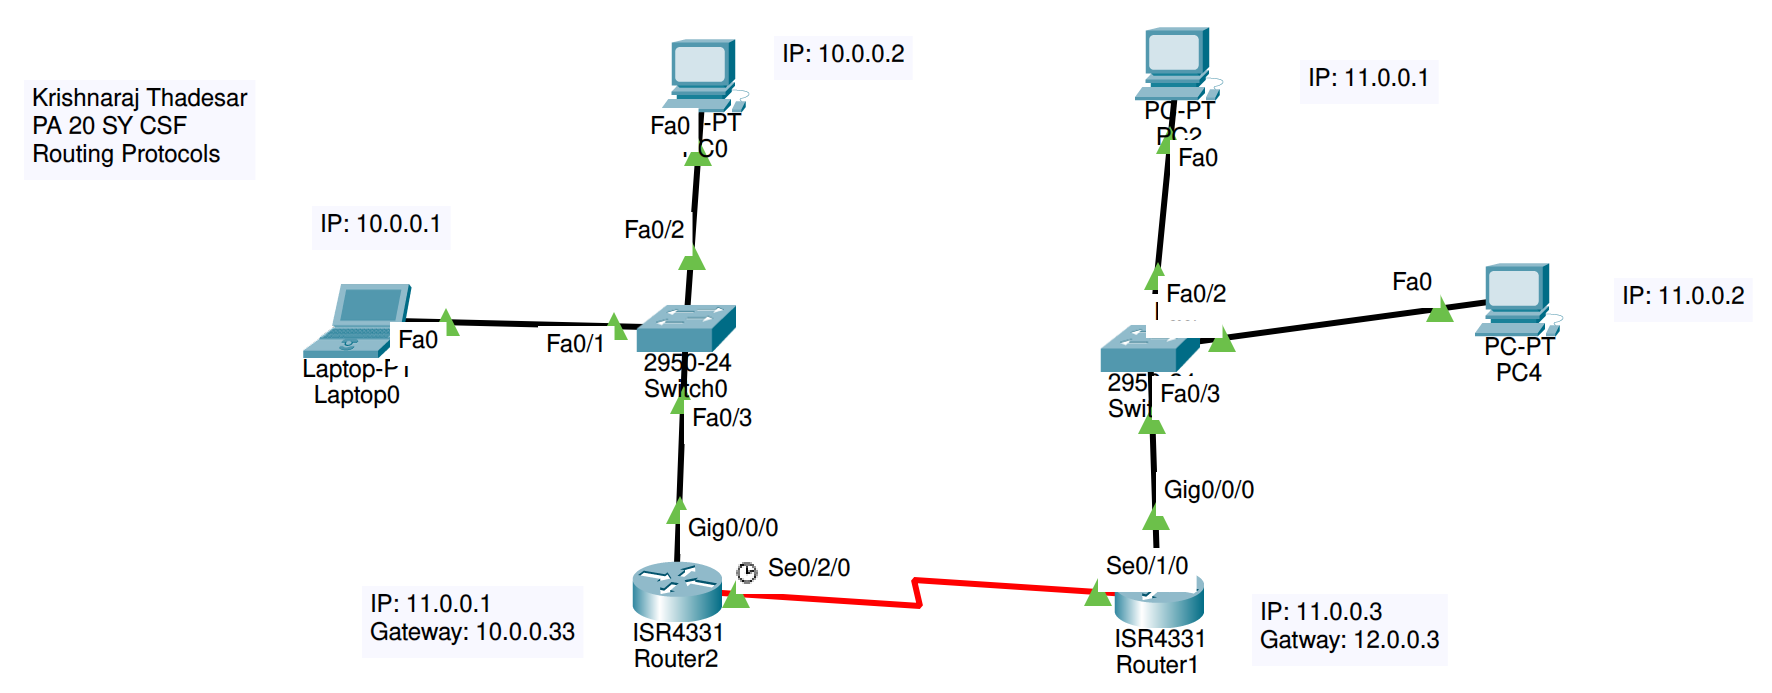
\includegraphics[scale=0.4]{../Screenshots/Assignment_7_screenshot.png}
\end{figure}


\section{Conclusion}
Thus routing Protocols were Executed on a simple LAN, and the connection was verified using the ping command. 3 Routing Protocols were executed successfully. RIP, OSPF and EIGRP. Their Differences were studied and understood. 
\end{document}